\subsection{Opgaver}

\begin{enumerate}
	\item Udregn følgende tal
	\begin{align*}
	2^4,&& 4^{-1},&& e^3, &&\Big(\frac{1}{2}\Big)^{3},&&\Big(\frac{1}{3}\Big)^{-3},&& 123^0.
	\end{align*}
	\item Udregn følgende tal
	\begin{align*}
	\log_2(256),&& \log_{10}(1000),&& \log_3\Big(\frac{1}{9}\Big),&& \ln(e^6),&&\log_{123}(1)
	\end{align*}
	\item Bestem fordoblings- eller halveringskonstanten for hver af de følgende funktioner
	\begin{align*}
	f(x)=\Big(\frac{1}{2}\Big)^x,&&g(x)=3e^x,&&h(x)=e^{-x}.
	\end{align*}
	\item Udregn følgende tal
	\begin{align*}
	\log_{10}(40)+\log_{10}(25),&&\log_{10}(40)-\log_{10}(4),&& \log_4(32)+\log_4\Big(\frac{1}{2}\Big)
	\end{align*}
	\item Udregn følgende tal
	\begin{align*}
	\ln(\sqrt{2}),&& \log_{10}(5^{3/2})+\frac{1}{2}\log_{10}(5)+\frac{1}{3}\log_{10}(64),&& \frac{1}{2}\log_5(4^2+9+10^2)
	\end{align*}
	\item Udregn følgende tal
	\begin{align*}
	e^{\ln(1)},&&2^{2+\log_2(10)},&& 10^{3\log_{10}(7)},&& 7^{-\log_7(9)},&& 4^{\log_2(3)}
	\end{align*}
	\item Bestem $a$ og $b$ så at $f(x)=ba^x$ går gennem punkterne $(1,2)$ og $(3,4)$.
	
	\item Løs ligningerne 
	\begin{align*}
	e^x=5,&& 10^{x^2}=100^x,&& 2^{x+1}=3,&& e^{x^2-45}=e^{-135}e^{19x}
	\end{align*}
	
	\item Løs ligningerne 
	\begin{align*}
	\ln(x)=4,&& 3\log_{10}(x)=\log_{10}(27),&&\ln(x)+\ln(x+2)=3\ln(2)
	\end{align*}
	
	\item Lad $f$ være en eksponential funktion med halveringskonstant $7$, som opfylder $f(3)=12$.
	\begin{enumerate}
		\item Bestem $f(-11)$
		\item Bestem $f(10)$
		\item Løs ligningen $f(x)=\frac{3}{2}$.
	\end{enumerate}
	
	\item Argumenter for, at det ikke giver mening at tage den naturlige logaritme af et negativt tal.
	
	\item Funktionen $f(x)=a^x$ har fordoblingskonstanten $ \ln(2^5) $. Bestem $a$.
	
	
	\item Bestem $a$ og $b$ så $f(x)=ba^x$ går gennem punkterne $(1,e^3)$ og $(3,e^7)$.
	
	\item \label{it:eks1} Figur~\ref{fig:eks1} viser graferne for tre forskellige eksponentialfunktioner. Hvilken af disse har den største fordoblingskonstant?
	
	\begin{figure}
		\centering
		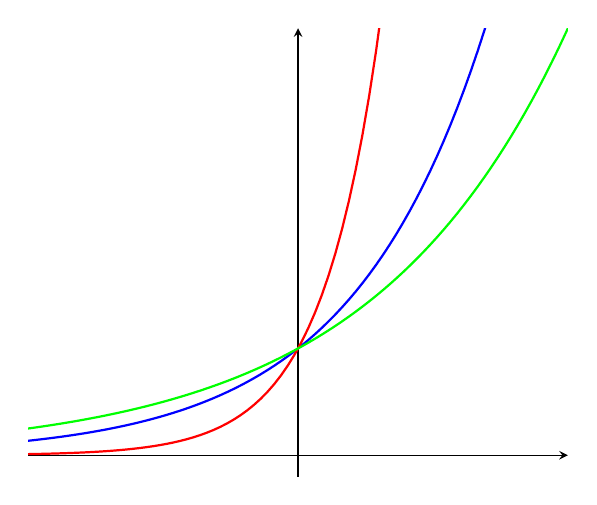
\begin{tikzpicture}
		\begin{axis}[xmin=-2,xmax=2,ymin=-0.2,ymax=4,axis x line=center,
		axis y line=center,ticks=none,restrict y to domain =0:20]
		\addplot[thick,blue, samples = 200] {exp(x)};
		\addplot[thick, red, samples = 200] {10^x};
		\addplot[thick, green, samples = 200] {2^x};
		\end{axis}
		\end{tikzpicture}
		\caption{Opgave~\ref{it:eks1}}
		\label{fig:eks1}
	\end{figure}


	\item Bestem halvveringskonstanten for funktionen $f(x)=e^{-2x}$
	
	
	\item Givet en eksponentialfunktion $f(x)=ba^x$ bestem $c$ og $d$ så $g(x)=cd^x$ er spejlingen af $f$ i $y$-aksen. (Hint: Symmetri om $y$-aksen er ensbetydende med at $f(-x)=g(x)$.)
	
	
	\item \label{it:eks2} Vis at 
	\begin{align*}
	\frac{\ln(a^y)}{\ln(a)}=y,\quad \textup{og}\quad a^{\frac{\ln(x)}{\ln(a)}}=x.
	\end{align*}
	Konkluder at
	\begin{align*}
	\log_a(x)=\frac{\ln(x)}{\ln(a)}.
	\end{align*}
	(Hint: til at vise den anden lighed brug at $ x=a^{\log_a(x)} $ på venstresiden.)
\end{enumerate}